\chapter{Ranking Algorithms}

\section{Task}
Typically, results returned from search engines are ranked so the more relevant search results first are featured on the top of the list. The general idea behind this is that, for a given website, a score is calculated for each word to indicate the importance of that word on such website.\\
As a query might consist of a union of a certain number of intersected searches, the score is calculated as follows:
\begin{itemize}
    \item Intersected Search: the score is a summation of the scores for each individual word in the search;
    \item Union Search: the score is taken as the maximum of the score for each part of the union search.
\end{itemize}
This score should then be used to order the results of a given query.

\section{Basic Approach}
For this task, the following ranking algorithms were introduced:
\begin{itemize}
    \item Term Frequency (TF)
    \item Term Frequency — Inverse Document Frequency (TFIDF)
    \item Okapi BM25 (which is discussed in detail on the Extensions section of this paper)
\end{itemize}
Please note that these consist of different implementations of the same aforementioned general idea: assigning a score to a website based on some metric of relevance.\newline
Research was conducted into the implementations of each of the ranking algorithms.

\subsection{Term Frequency}
The TF is simply this: given a word and a document (which in this case, is a webpage), how many times does a word appear on that document? \citep{luhn1957statistical}\\
Even though there are various implementations on this basic formula, the $TF$ formula settled on in the end was:\\
Let
\begin{itemize}
    \item $TF$ be the term frequency
    \item $f$ be number of occurrences of a given word on the website
    \item $w$ be the total number of words on that website
\end{itemize}
We have:
\begin{align}
    TF &= \frac{f}{w}
    \label{eq:TF}
\end{align}
Such formula enabled us to add a layer of normalisation on the score, as a word occurring 10 times on a 50-word-long website has a different significance to a word appearing 10 times on a 500-word-long website.

\subsection{Term Frequency — Inverse Document Frequency}
Before the $TFIDF$ algorithm can be discussed, the idea behind "Inverse Document Frequency" must be explained.\\
The idea behind the inverse document frequency is that, while the number of times a word appears on a webpage is a good indication of how important that word is to that webpage, there are many common words such as "the", "and", "this", etc., that will inevitably appear multiple times on a website and will therefore skew the score of any kind of score based on term frequency \citep{Jones72astatistical}.
The inverse document frequency formula is designed to take this into account and is calculated as follows:\newline
Let
\begin{itemize}
    \item $IDF$ be the inverse document frequency
    \item $s$ be number of websites in the search engine index
    \item $sw$ number of websites containing the word
\end{itemize}
We have:
\begin{align}
    IDF &= log_{2}\bigg(\frac{s}{sw}\bigg)
    \label{eq:IDF}
\end{align}
Taking the $log$ of this ratio means that, the more times a word appears on a website in the database, the closer the $IDF$ gets to $0$, and a word that appears on every website in the database is awarded an $IDF$ value of $0$.\\
In other words, common words that are likely to appear on multiple (if not all) websites will have no impact on the ranking score. With that in mind, the meaning behind the $TFIDF$ ranking algorithm becomes clear. By (\ref{eq:TF}) and (\ref{eq:IDF}), the $TFIDF$ score is calculated as follows:
\begin{align*}
    TFIDF = TF \times IDF
\end{align*}
The $TF$ score judges the relevance of the word to the website, and the $IDF$ is a weighting to adjust for common words. Very common words are awarded a $TFIDF$ score of 0 (or close to 0) and therefore give no impact in intersected searches.\newline
It was also decided that the various implementations of {\tt Score} classes created would be solely responsible for the calculations.

\section{Technical Description}
As per the task description, a generalised {\tt Score} interface was created with only one method — {\tt getScore} — which performs the score calculation for the given word with the given website, taking the following parameters:
\begin{itemize}
    \item {\tt @param word}: a word from the search query
    \item {\tt @param site}: the website being scored against the search string
    \item {\tt @param index}: the index of websites
\end{itemize}
Each of the below classes implement this interface. In addition to this, the {\tt rankWebsites} method was added to the {\tt QueryHandler}. That essentially takes one of the given ranking algorithms and scores the websites relevant to the query and then order them from highest to lowest. This method will also be used by the OkapiBM25 algorithm.

\begin{figure}[t]
    \centering
    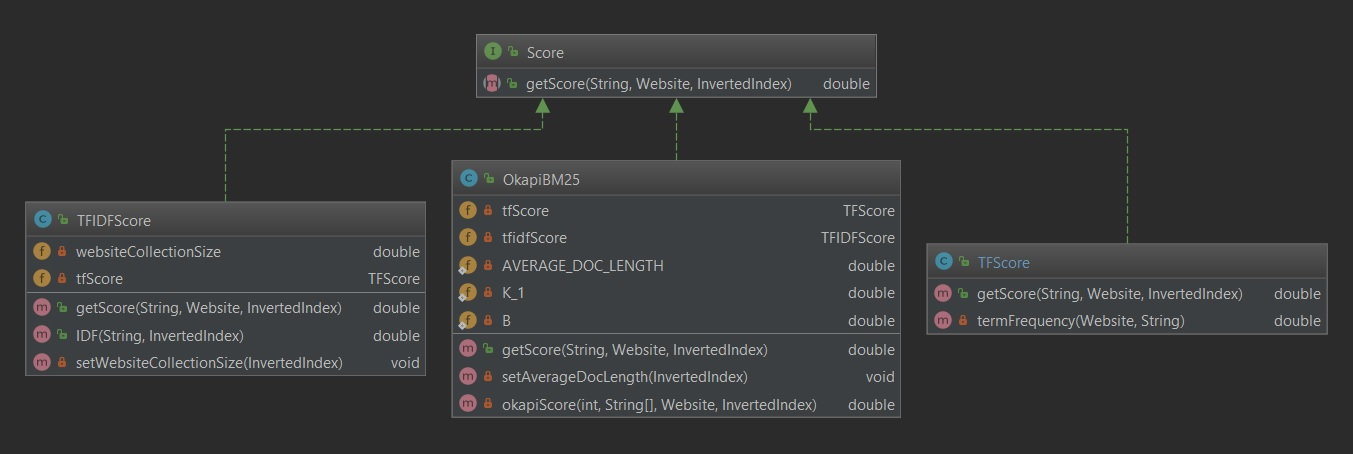
\includegraphics[width=\textwidth]{figures/diagram-score}
    \caption{UML Diagram for the Software Architecture of Score data structures.}
    \label{fig:score:uml}
\end{figure}

\subsection{{\tt TFScore} class}
The {\tt TFScore} class was the simplest of the three classes to implement, as shown in Figure \ref{fig:score:uml}.
Due to the changes made to the {\tt FileHelper} class — namely, that no website that lacks a title or words can be created — it's not possible for there to be a divide by zero error, so no steps were made in this method to account for it.

\subsection{{\tt TFIDFScore} class}
As the $TFIDF$ makes use of the $TF$ calculation, the {\tt TFIDFScore} class was given a field of type {\tt TFScore} with which to call methods on as needed, rather than creating a new object each time it was required. Helper methods were added to deal with the different aspects of the calculation, i.e. the $IDF$ and the number of websites in the search engine index. Also, in order to enable any {\tt Index} to work with this implementation, a helper method was added there — {\tt provideIndex} — which returns a {\tt Collection<Website>}, much needed to compute this. The number of websites was built from the {\tt Index Map<String, Website>}. Such implementation makes use of the fact that a {\tt HashSet} allows no duplicates in order to calculate the number of distinct websites in the {\tt Index}.\\
Again, the {\tt getScore} method only handles the multiplication.

\section{Testing considerations}
The mathematical correctness of the score calculations were verified using unit tests, which can be found in the ScoreTest.java file.\\
The positive testing approach was applied in this context.
The set up comprised of building a small number of websites, which allowed for the score values of various words on various websites to be calculated manually and compared to the results of the {\tt getScore} method.\\
Each test covered one class, and the individual tests were determined using the standard white-box coverage considerations. For the tests on the {\tt TFIDFScore} class, a comparison was also included to confirm that a word occurring once on more than one site will have a lower score than a word occurring once on just one site.\\
The application of the algorithms were tested in the RankScoreTest.java file. White-box and positive testing were used in these tests. The test checked whether ranking algorithm $TF$ and $TFIDF$ would rank the websites correctly. The two ranking algorithms were testing websites which were set up specifically for the tests to allow easier prediction of how the ranking should be. Two websites in the {\tt setUp} was made to create noise, to see how the algorithms would react to them.

\section{Reflection}
After implementing the two different ranking algorithms and testing their implication it was possible to compare the different results they provided. While the $TF$ algorithm sums together the term frequency of each word in the search query, the $TFIDF$ algorithm also considers the relative frequency of each of the words in the search query appearing across the collection of websites on which the search is performed. This means that if the search query would consist of, e.g. "Queen of Denmark", the $TFIDF$ ranking algorithm would provide more relevant results than the $TF$ algorithm, because one could assume that the word "of" would appear significantly more often across different websites, than words "Queen" or "Denmark". Therefore, while the unit tests were used to verify the mathmatical correctness of the algorithms, the test in {\tt RankScoreTest} was also set to demonstrate the potential relationship between the search query and the background of the rest of the websites in an abstract and simplified manner.\\
Based on the theoretical assumptions on the relevance of the two algorithms when applied to querying, and their behaviour in the {\tt RankScoreTest}, it can be concluded that the $TFIDF$ is the most relevant to as it provides a more appropriate result to the user's search query.